\documentclass[11pt, oneside, titlepage]{jarticle}
\usepackage[margin=25truemm]{geometry}
\geometry{letterpaper}
\usepackage[dvipdfmx]{graphicx}
\usepackage[cc]{titlepic}
\usepackage{url}
% hyperrefとbreakurlの設定を修正
%\usepackage[dvipdfmx,unicode,bookmarks=true,bookmarksnumbered=true,bookmarksopen=true,colorlinks=true,linkcolor=blue,urlcolor=blue]{hyperref}
\usepackage{here}
\usepackage{float}
\usepackage{ascmac}
\usepackage{amsmath}
\usepackage{amssymb}
\usepackage{ulem}
\def\UrlBreaks{\do\.\do\@\do\\\do\/\do\!\do\_\do\|\do\;\do\>\do\]\do\)\do\,\do\?\do\'\do+\do\=\do\#}
\usepackage{mathtools}
\usepackage{listings,jvlisting}
\lstset{
  basicstyle={\ttfamily},
  identifierstyle={\small},
  commentstyle={\smallitshape},
  keywordstyle={\small\bfseries},
  ndkeywordstyle={\small},
  stringstyle={\small\ttfamily},
  frame={tb},
  breaklines=true,
  columns=[l]{fullflexible},
  numbers=left,
  xrightmargin=0zw,
  xleftmargin=3zw,
  numberstyle={\scriptsize},
  stepnumber=1,
  numbersep=1zw,
  lineskip=-0.5ex
}
\usepackage{float} 
\renewcommand{\lstlistingname}{プログラム}
\newcommand{\diff}{\mathrm{d}}
\usepackage{latexsym}
\def\qed{\hfill $\Box$}
\usepackage[version=3]{mhchem}
\title{ \large{2024A・機械情報冬学期演習・自主プロジェクト}\\
\vspace{1cm}
\Huge{卓球ロボット HARIMOTO}}
\author{東京大学工学部機械情報工学科3年 \\
学籍番号: 03-240281 \\
氏名: 椿 道智}
\titlepic{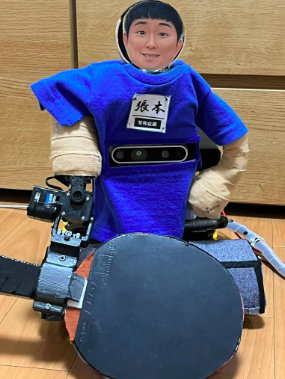
\includegraphics[width=10cm]{figures/HARIMOTO.png}}
\begin{document}
\maketitle
\section{概要}
本プロジェクトでは,卓球台上で稼働可能な卓球ロボット HARIMOTO(以下,単に「ロボット」という.)を製作した.ロボットは,「プッシュ卓球打ち(=温泉卓球打ち)」「ドライブ打ち」の二種類の打撃方法により,投げた卓球ボールに対して,タイミングよく振ることができる.単に,打撃制御や画像処理をするだけではなく,ボールが返球された際の「チョレイ」効果音や外装の工夫により,実際の張本感を出し,ユーザ側が楽しめるようにも工夫した.

ソフトウェア面では,アームの動作(卓球ボールの打撃),D435iによる画像認識(卓球ボールの認識),軌道予測,メカナムホイールの制御,音声再生を行った.機械工学少人数ゼミ(岡田慧教授ゼミ)や知能ロボット演習(機械情報冬学期演習)で学んだeuslisp・ROS noeticを用いてシステムを組んだ.

ハードウェア面では,4自由度アームの設計・制作,ラケットや服,左腕や靴など外装の製作・塗装を行った.また,アームやホイールは,知能ロボット演習で用いたjedyと同じ,近藤のサーボモータやメカナムホイールを用いて製作した.

\section{動機・背景}
私は,卓球サークルに所属しているということもあり,卓球が好きなので,卓球をするロボットを製作することにした.卓球ロボットといえば,卓球台の外に大きなパラレルリンクを設置して返球させる手法が従来研究開発されてきた.しかし,そのような手法では,設置のスペースのコスト,パラレルリンクの設計/制御の難しさのコスト,巨大さゆえの値段的なコストなど様々なコスト面の課題があると考えた.そこで,本プロジェクトでは,それとは逆に「省スペース」「シリアルリンク」「低額」をコンセプトに新しい卓球ロボットを制作することを目標にした.

\section{コンセプト}
卓球選手の戦型は,前陣(速攻)型・中陣型・後陣型の3種類に大別される.それぞれ,卓球台のエンドラインから0mから1m離れた場所から打つ,1mから2m離れた場所から打つ,2m以上下がった場所から打つ戦型である.この内,前陣型は,卓球台にほとんどくっついて打つような戦型なので,ボールの着地直後にラケットをボールに接触させて返球させる.

前陣型の戦型が存在するということは,理論上は,(エッジボールなどを除いたほとんどのボールは),台から離れなくても「台上」で返球可能であり,この「前陣型」戦型が,私が今回「卓球台上」で返球するロボットが製作可能だと考えた根拠である.さらに,ほとんどのボールに対して着地直後の返球をするので,ラケットの存在する高さも低い範囲に制限できるというメリットがある.一方で,前陣「速攻」型とも言われるように,前陣でプレーをすることになると,ボールの返球までの時間的な猶予が少なくなり,素早い認識と判断が求められ,これが本プロジェクトの難点の1つにもなっている.

\section{環境構築・実行方法(Github)}
本プロジェクトにかかるすべてのソースコードと自作パーツのモデルは, \url{https://github.com/Michi-Tsubaki/ping-pong-robot}で公開している.
\begin{screen}
git clone https://github.com/Michi-Tsubaki/ping-pong-robot.git
\end{screen}

なお,本レポート内でも,説明に必要な範囲でソースコードを参照する.

\subsection{実行方法}
\begin{screen}
cd ~/ping-pong-robot\\
source devel/setup.bash \\
roslaunch HARIMOTO all.launch \#画像処理やアームコントローラのノードを起動
\end{screen}
\begin{screen}
cd ~/ping-pong-robot\\
source devel/setup.bash \\
roscd HARIMOTO/src \\
emacs -nw 
M+x shell
source ~/ping-pong-robot/devel/setup.bash
roslaunch HARIMOTO all.launch \#画像処理やアームコントローラのノードを起動
\end{screen}
\section{機能}
ロボットは,以下の機能を備えている.
\begin{enumerate}
\item {\bf 着地予測して打つ} \\
 空間を「近距離」「中間距離」「遠距離」の3つの空間に分け,空間によって着地までの猶予が異なることから,前者から,予測せずに直ちに打つ,速度の生データから着地予測して打つ,速度にフィルタ処理を施して予測位置に移動して打つ,を機動的に使い分けながら打撃のタイミングを決めている.
\item {\bf 打つ→チョレイ} \\
 4自由度ながらも力強く打てるように試行錯誤した打撃関数を作成した(引数は高さ).上手く打てると,「チョレイ」と叫ぶ仕様にいなっている.
\item {\bf 打撃モード} \\
 開始時のアームの高さに応じて「プッシュ打ち」モードと「ドライブ打ち」モードを起動することができる.
\item {\bf 警告} \\
 サーボモータに長時間負荷をかけ続けると故障の原因となるため,起動後2分後と5分後に「腕が疲れてきたよ」という警告音を発し,プログラムの停止を促している.
\end{enumerate}
\section{システム構成}
ロボットのシステム構成は,図\ref{system}の通りである.ロボットは,4自由度ロボットアーム・Interl d435 depthカメラ・メカナムホイール・スピーカーから構成される.これらと,main.l(制御アルゴリズム),画像処理のノード(detect\_ball.launchで起動)をros topicでつなぐことでシステムが構成されている.詳細はros topicとros nodeのグラフ(rqtグラフ)を図\ref{rqt}に示すが,字が小さくて読みづらい.
\begin{figure}[H]
\centering
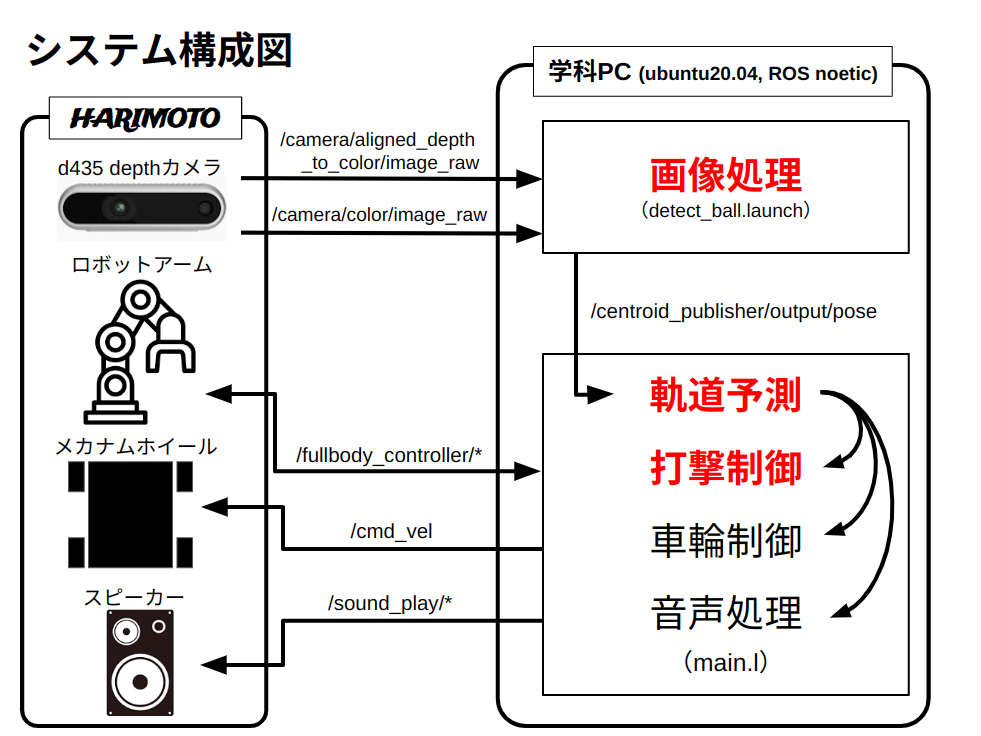
\includegraphics[width=12cm]{figures/system.png}
\caption{システム構成図}
\label{system}
\end{figure}
\begin{figure}[H]
\centering
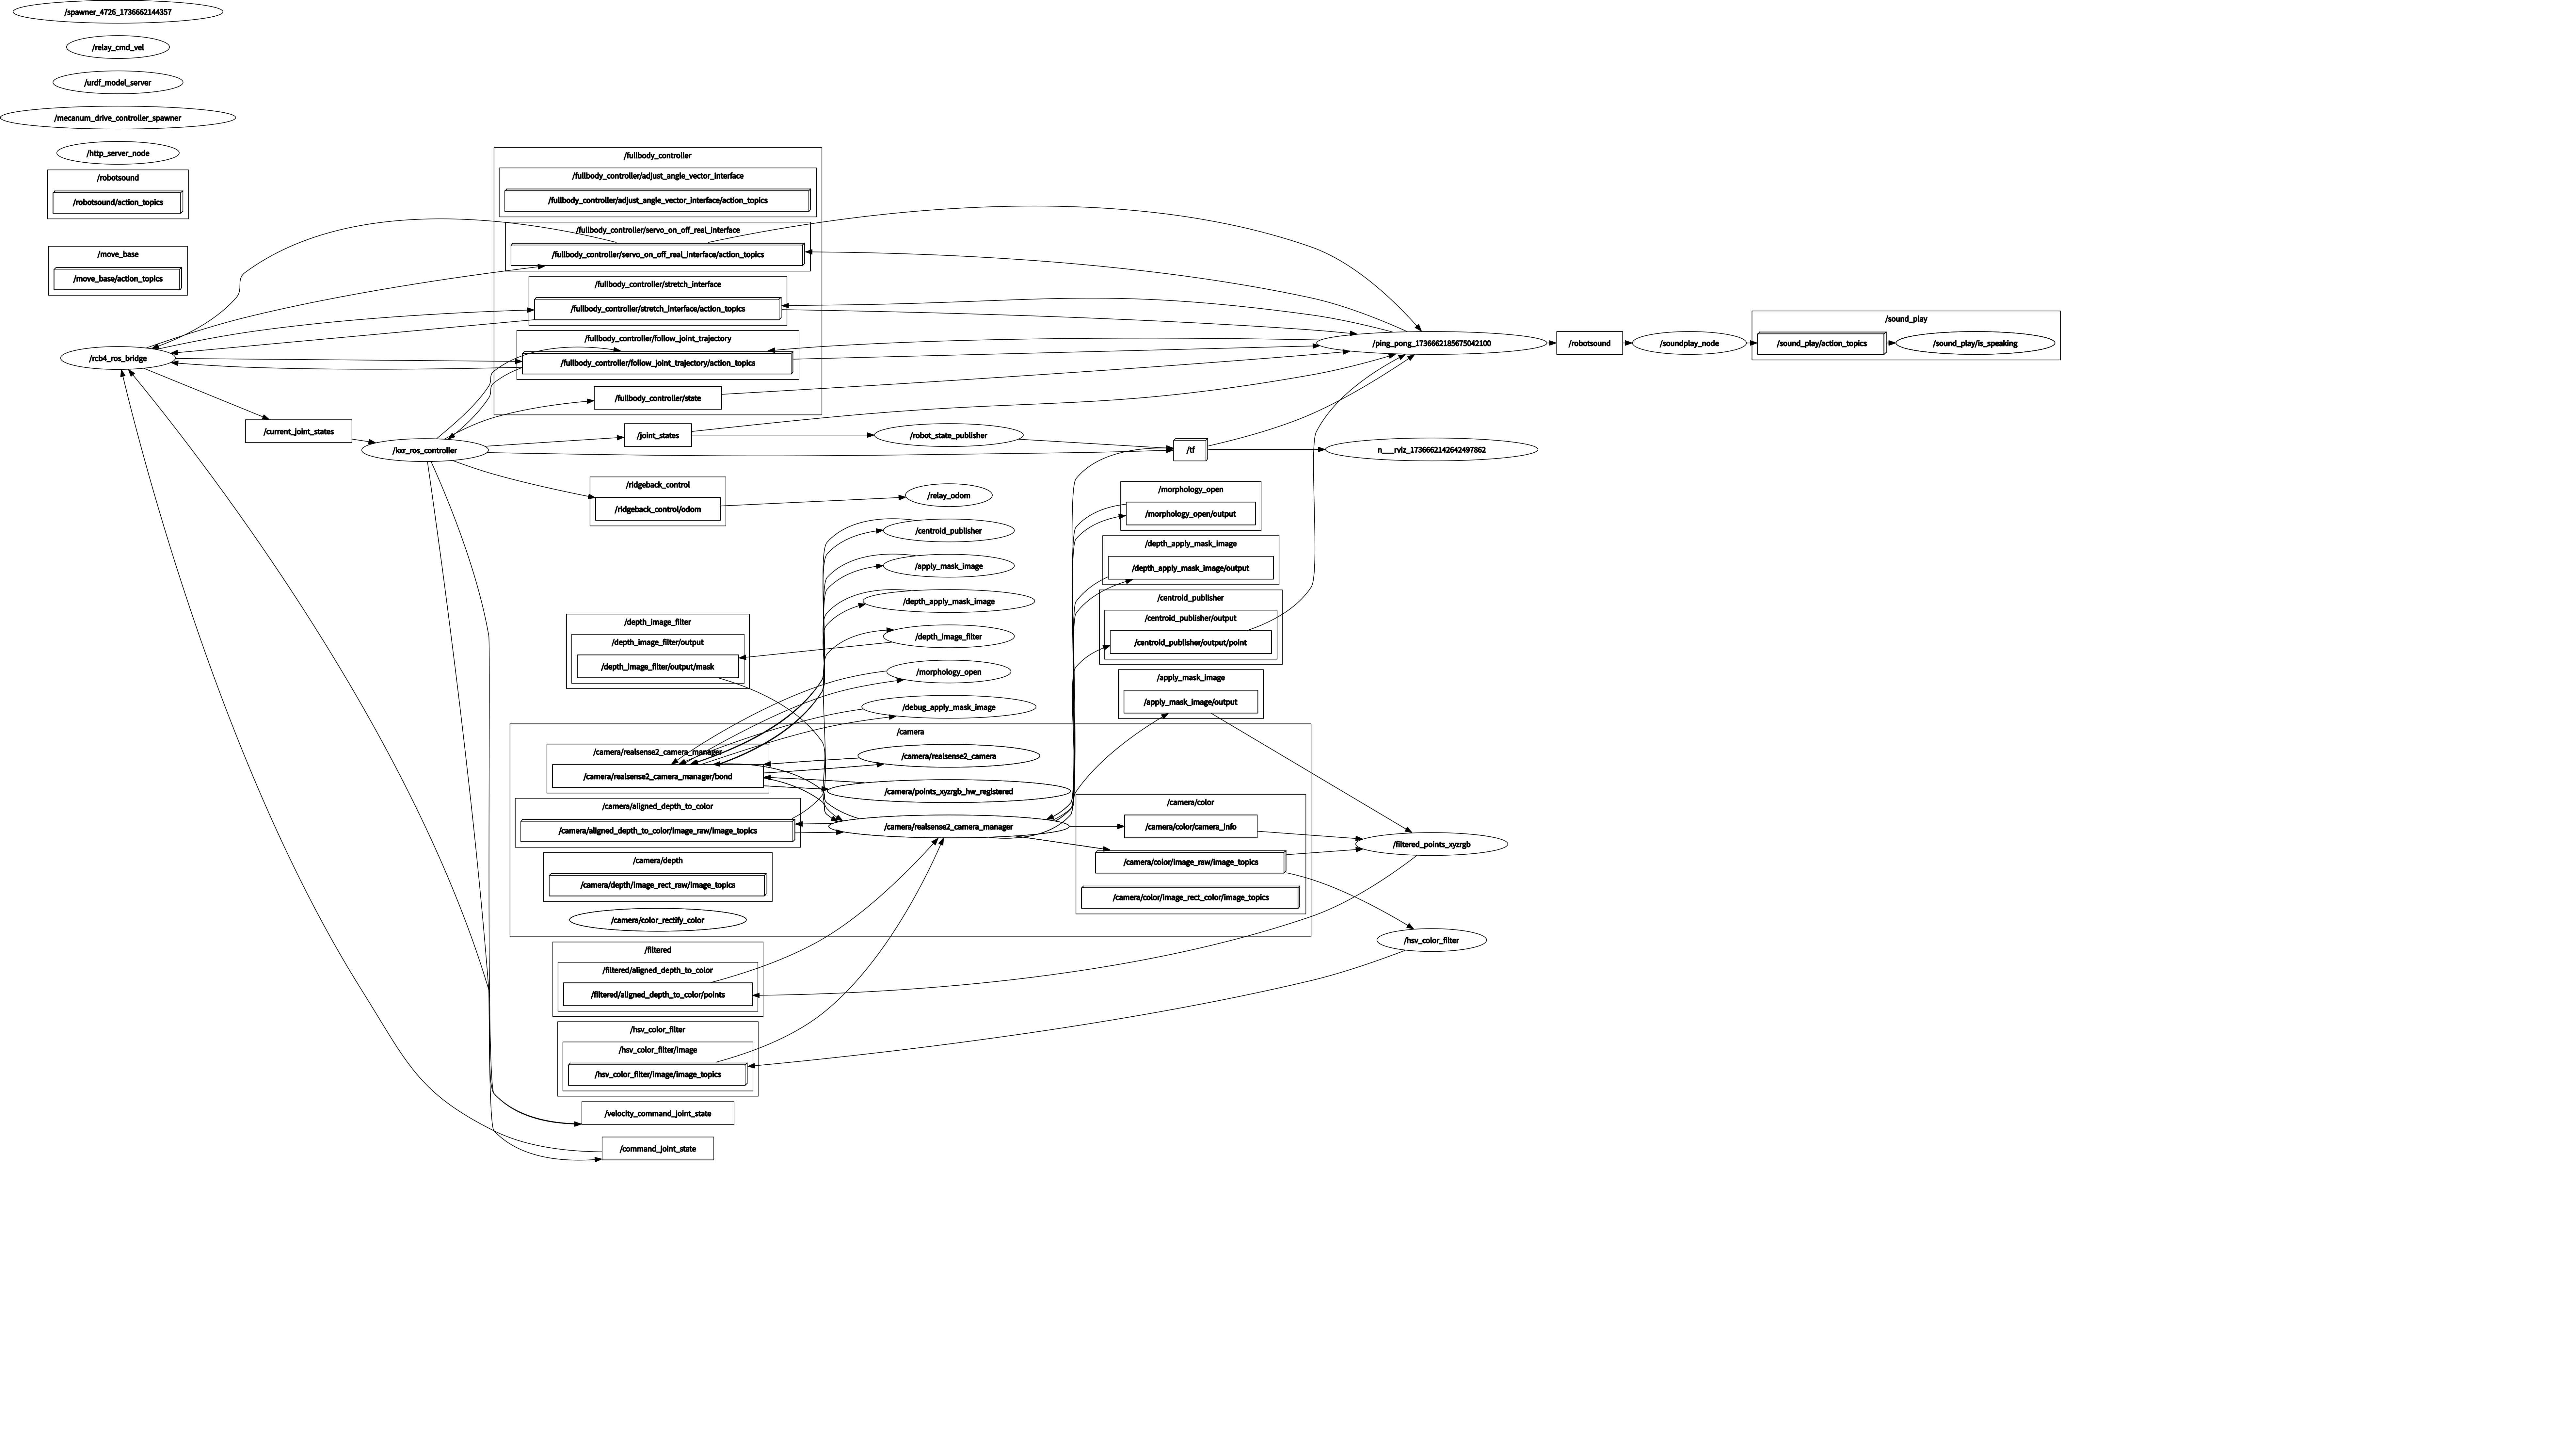
\includegraphics[width=15cm]{figures/rosgraph.png}
\caption{rqt\_graph}
\label{rqt}
\end{figure}
\section{ソフトウェア}
\subsection{統合制御アルゴリズム}
本節では,打撃(アーム)・軌道予測・画像認識・メカナム制御のサブルーチンを統合し,卓球ボールの返球を実現するアルゴリズムについて説明する.
\subsection{打撃}
本節では,卓球ロボットHARIMOTOの4軸ロボットアームによる打撃の方法について説明する.
\subsection{軌道予測}
\subsection{画像認識}
本節では,Intel RealSense Depth Camera D435iを用いたボールの中心位置の取得するプログラムついて説明する.
「HSVカラーフィルタ」で

苦労した点・新旧も含めて説明する.\cite{detect2}
\subsection{メカナムホイール制御}
本節では,メカナムホイールの制御プログラムについて説明する.\cite{mecanum}
\subsection{音声再生}
本節では,音声に関する実装について説明する.\cite{sound}
\section{ロボットモデル・ハードウェア・メカニクス}
\subsection{ロボットモデル}
本節では,自作パーツを含むロボットのアセンブリからURDFの製作について説明する
\subsection{ロボット設計・製作}
本節では,ロボット全体の設計思想・製作,自作パーツの設計について説明する.

\subsection{外装}

\section{オリジナリティ・工夫}

\section{気づいたこと}

\section{今後に向けて}

\section{作業記録(参考)}
本プロジェクトの進捗は,\url{http://github.com/Michi-Tsubaki/ping-pong-robot/issues}で管理した.詳細は,そちらを参照してほしい.ここでは,その要点を当初の計画と比較しながら振り返る.
\section{謝辞}
本プロジェクトに取り組むに際し,スケッチに対するフィードバック,部品の貸出提供,都度の助言を下さった,自主プロA班の矢野倉助教,小島講師,3Dプリンタの使用でご協力下さったメカノデザイン工房の方々,アドバイスをくれた機械情報工学科3年の皆さんに御礼申し上げます.

\begin{thebibliography}{9}
\bibitem{detect2} 
Michi-Tsubaki, ``recognize\_wound.launch,'' jsk\_demosm GitHub. [Online]. Available: 
\path{https://github.com/Michi-Tsubaki/jsk_demos/blob/jsk_2024_10_semi/jsk_2024_10_semi/pr2_surgery/launch/recognize_wound.launch}

\bibitem{mecanum} 
iory, ``[jedy\_bringup] support mecanum drive using ridgeback\_control \#2,'' robot-programming, GitHub. [Online]. Available: 
\path{https://github.com/iory/robot-programming/pull/2}

\bibitem{sound} 
jsk-ros-pkg, ``speak.l,'' jsk\_pr2eus, GitHub. [Online]. Available: 
\path{https://github.com/jsk-ros-pkg/jsk_pr2eus/blob/master/pr2eus/speak.l}
\end{thebibliography}

\end{document}
